\documentclass{article}
\usepackage{CJKutf8}
\usepackage{multicol}
% Packages
\usepackage{lipsum} % For generating dummy text
\usepackage[top=1in, bottom=1in, left=1in, right=1in]{geometry}
\usepackage{hyperref}
\usepackage{pgfplots}
\usepackage{caption}
\captionsetup{font=small}
\usepackage{standalone}
\usepackage{listings}
\usepackage{xcolor} % For setting colors
\usepackage{amssymb}
\usepackage{amsmath}
\usepackage{algorithm}
\usepackage{algpseudocode}
\usepackage{afterpage}
\usepackage{placeins}
\usepackage{tikz}
\usepackage{enumitem}
\lstset{
  language=[LaTeX]TeX,
  breaklines=true,
  basicstyle=\ttfamily\small,
  keywordstyle=\color{blue},
  commentstyle=\color{green},
  backgroundcolor=\color{gray!10},
  frame=single,
  showspaces=false,
  showstringspaces=false,
}
\pgfplotsset{compat=1.17} % Use this to ensure compatibility with newer features
\setlength{\parskip}{6pt}
% Title and author
\title{Autonomous competence identification protocol}

\author{Tim Pechersky}


\begin{document}
\begin{CJK}{UTF8}{gbsn}

    % \twocolumn
    \maketitle


    \begin{abstract}
        This paper introduces a novel protocol for establishing ranking systems in Decentralized Autonomous Organizations (DAOs) and consensus-building protocols. Leveraging cryptographic and social science insights, the protocol enables autonomous decision-making in trustless environments based on agent interactions. A real-world case study demonstrates the protocol's potential to achieve high participation and retention rates, even without explicit incentives. The proposed protocol addresses key challenges in autonomous governance, such as low participation, centralization, and lack of commitment mechanisms, by fostering a more engaging, equitable, and secure decision-making process. It also has potential applications in various domains beyond DAOs, including decentralized social networks, academic research, and online education.
    \end{abstract}
    \begin{multicols}{2}

        \section{Introduction}

        The quest for consensus, a cornerstone of collective decision-making, has deep historical roots. From the ancient Chinese concept of \textit{zhongyong} {\CJKfamily{bsmi}
            中庸}, advocating for moderation and balance in governance, to the Roman Republic's emphasis on \textit{senatus consulta} (senate decrees) reached through deliberation and compromise, societies have long grappled with the challenge of aligning diverse perspectives towards a common goal. The study of these historical precedents continues to inform modern approaches to consensus \cite{Andersen2019} \cite{Frederic2014}. \\
        The pursuit of consensus has gained renewed significance in the digital age. Originating from the Bitcoin whitepaper \cite{Satoshi}, blockchain technology fundamentally seeks consensus and establishes trustless system through cryptographic signatures. While significant progress has been made in developing efficient Byzantine Fault Tolerance (BFT) algorithms for reaching consensus on verifiable data \cite{Genrui2023}, the challenge of achieving consensus on subjective or non-deterministic matters within DAOs \cite{Hassan2021} remains a complex issue \cite{Shuai2019}\cite{Rainer2023}. This has led some researchers to question the ability of autonomous organizations to overcome the hierarchical issues present in today's society \cite{Marcella2016} \cite{Xuan2024}.   \\
        This paper introduces a novel protocol designed to bridge the gap between formally verifiable, automated consensus and subjective human decision-making. By qualifying participants based on their ability to represent a group's interests and intents, our protocol aims to achieve consensus even for subjective matters. This protocol serves as a foundational building block for designing ranking systems applicable to both computational and social networks, addressing long-standing governance issues such as agenda manipulation  \cite{McKelvey1976}.\\
        The main objectives of this research are to:

        \begin{itemize}[nosep]
            \item Propose a methodology for creating a ranking system in a trustless environment
            \item Review potential attack vectors and resistance mechanisms.
            \item Provide a case study of an existing use case.
            \item Discuss potential economic models for the practical utilization of such competence frameworks.
        \end{itemize}
        We begin by reviewing existing consensus mechanisms and their limitations, focusing on DAOs and their governance mechanisms. We then introduce our proposed protocol, followed by a discussion of its implementation and potential economic models. Finally, we present a case study of an existing use case and conclude with a discussion of future research directions.

        \section{Background}
        % Write your methodology here
        Neither decentralized autonomous governance nor consensus protocols cannot be defined completely through cyber-physical systems' (CPS) \cite{Lee2008} methodology, as such organizations involve social aspects. Nevertheless, an end goal for any autonomous governance is to operate CPS, which might in future evolve enough to fully automate the management of manufacturing plants, data centers and other cyber-physical infrastructure key components. In this context any kind of IT governance system can be seen through the methodology of Cyber-Physical-Social-System (CPSS) \cite{Fei2016} which attempts to account for the social aspect of intellectual management in a post-AI age.

        \paragraph{Parallel management} is a concept introduced recently by researchers exploring management perspectives in the cyber age \cite{Wang2022}, focused on highly efficient and autonomous decision making and feedback processes. These management frameworks proposed are modeling DAOs as a core element of such CPSS and openly discuss the need for multidimensional indexes and foundational models to measure knowledge works \cite{Juanjuan2023}. References to DAOs as an instrument within CPSS and parallel management are a recognition by academic research of a need for such organizational structures for more efficient management process in the future. As per discussion for parallel management \cite{Wang2022}, there is also a need for a robust mechanism for reinforcing the informational and intellectual capabilities of organizations, enabling them to effectively benchmark the performance of AI enabled agents against humans in various tasks and aspects of governance and management.

        \paragraphThe {Nakamoto Coefficient} is another newly introduced concept that helps to measure the decentralization of a protocol \cite{Balaji2017}. It is defined as \textit{how many entities one would need to to be compromised to control entire system} and it can be used as a decentralization criteria.

        \paragraph{Traditional governance models} have a long-standing backlog of unresolved problems. One prominent one is agenda manipulation \cite{McKelvey1976}, that should be addressed well to ensure high reliability of organizations in autonomous systems. Participation rates (turnout) is also being studied and seen to be in decline in major countries over past decades \cite{Lawrence23}\cite{Filip24}


        \subsection{Consensus Layer}
        Blockchain is a distributed and decentralized network that follows some particular consensus protocol in order to maintain a continuous sequence, or chain of blocks\cite{Merlinda2019}, where each new block consists of a digital entry to a united ledger book. First introduced through the launch of Bitcoin\cite{Satoshi}, it has grown into an industry where multiple approaches and protocols were developed, and the initial ability to write records in to ledger book was elaborated with the ability to write code in ledger records such that it can change states of book itself.
        The blockchain's governance plays a critical role in any blockchain protocol and can be summarized as consisting of Validators, Users, Governance Mechanisms and core developer community; In this context a blockchain network is analogous to an organization, consisting of validators (employees), protocols, and governance structure, whose activity results in services provided to users who have some input through deciding to pay for using the protocol.

        The contrast between traditional organization and blockchain governance is CSP-friendly automation. Such blockchains are designed to follow some pre-determined rules to maintain the distributed ledger with no need for human stakeholder decisions over regular operations. which are automated by running specific software applications (nodes) that act on behalf of stakeholder.
        These however only work well until protocol changes are desired or some vulnerability is found which leads to a collective decision of stakeholders for stepping-off the protocol rules \cite{Liu2021} for at least one block. Such occasions are generally called hard-forks, and have the characteristic that coordinated consensus between node operators changes their protocol rules to move away from the existing logic. The "fork" in this context describes a split of consensus leading to two possible ledger book states which are not compatible. \\
        Consensus layer protocols also have the underlying node operator community whichis  incentive-driven. Studies have been done on Nash Equilibrium \cite{Nida2020} while the real situation for Ethereum is that Miner Extracted Value is shown \cite{Philip2019} to be a realistic threat to protocol-level security, that comes down to affecting applications such as decentralized exchanges. The same paper also observes that agents pursuing MEV can achieve cooperative equilibrium in terms of priority gas auctions. \\
        "Ethereum Proof-of-Stake Consensus Layer: Participation and Decentralization research" \cite{Dominic2023} has shown that practical Nakamoto coefficient numbers in automated consensus engines such as PoS and Pow (Proof of Stake and Work respectively) have stabilized on very low numbers of less then 5 entities standing behind the whole pool of validators and miners, and seem not to show any positive dynamics.

        % \paragraph{}
        \subsection{Application Layer}
        While research in CPSS points out demand for DAOs as solution \cite{Fei2016}\cite{Wang2022}\cite{Juanjuan2023}, the ability of DAOs to perform well and be competitive, is under question, as many researchers point out associated problems \cite{Rainer2023}\cite{Marcella2016}\cite{Xuan2024}.  \\An empirical Study of On-Chain Governance conducted by Rainer Feichtinger et. al. \cite{Rainer2023} shows low Nakamoto Coefficient numbers, however comparing it with Consensus Layer research \cite{Dominic2023} we can conclude there is a positive dynamic in the Nakamoto coefficient over time in DAOs, compared with its absence for the consensus layer. The same research\cite{Rainer2023} also showed that the Gini coefficients\cite{Lidia2012} are high in the DAOs analyzed, reaching 0.888-1 for direct holders and 0.667-0.980 range when counting delegates, and that participation rates in DAOs are low. Out of four DAOs analyzed (Compound, Uniswap, ENS and Gitcoin), none of them are showing positive dynamics in participation rate over time, and mean numbers for participation even amongst delegates are in range of 1.1-9.9\% of total delegated accounts. Similar centralization problems are shown in \cite{Robin22}, which concludes that two DAOs, namely Compound and Uniswap DeFi protocols in fact are extremely centralized and controlled by a very small number of addresses, while their governance systems are looking more like a shareholder meeting, where a small number of large investors represents actual governing power.


        Another highlighted problem can be seen in the voting participation quorum thresholds, which are low. For example, Compound DAO quorum requires only 400,000 \cite{CompDAO} votes out of 10,00,000 total token supply \cite{CompToken}, which is only 4\%, yet in practice some proposals fail to reach even this low threshold the first time and have to re-submit \cite{CompProp232}\cite{CompProp237}. To illustrate the problem further, quorum requirements of a few high value DAOs are illustrated in Table \ref*{table:dao-metrics}. Ethereum PoS validator count is also shown to represent a consensus level engine specifics. Such low quorum requirements are directly explainable by low participation rates, and already have a record of quorum attacks \cite{AragonBlog}\cite{rhizoo2023} that were exploiting this weakness, while in high participation rate consensus layer systems, such as PoS and PoW, the financial incentives towards participation are shown not just to negatively impact Nakamoto coefficients, but have also shown that any network node must be seen as a rational agent which may diverge from the collective interest \cite{Philip2019}. Even so, the technical complexity and network requirements result in an effective quorum attack threshold of only 19\% for the whole Ethereum L1 at the time of writing.
        % \end{multicols}
        % \afterpage{
        % \onecolumn
        % \clearpage
        \begin{table}[ht]
    \centering
    \caption{DAO Minimal Quorums}
    \label{table:dao-metrics}
    \begin{tabular}{|l|l|l|l|}
    \hline
    \textbf{Name of DAO} & \textbf{Total Supply} & \textbf{Quorum} & \textbf{Threshold (\%)} \\ \hline
    Compound             & 10e6            & 400e3             & 4\%                     \\ \hline
    Uniswap              & 1e9             & 40e6              & 4\%                     \\ \hline
    ENS                  & 100e6           & 1e6               & 1\%                     \\ \hline
    Arbitrum             & 10e9            & 300e6-500e6       & 3-5\%                   \\ \hline
    Lido                 & 1e9             & 50e6              & 5\%                     \\ \hline
    \end{tabular}
    \end{table}
        % }
        % \begin{multicols}{2}
        % \twocolumn
        % \paragraph{}
        \subsection{Comparing two above}
        DAOs ultimately are just an abstraction layer on top of Consensus, allowing blockchain users to abstract away from calculations intensity onto smart contract programming and therefore more versatile, dynamic governance systems that can rely on underlying consensus security guarantees. Difference however also lies in implementation specifics: while Consensus layers do provide participation incentives, the application layer organization might not propose such at all, instead providing a means to make a governance decisions that are profitable on their own. \\ Analyzing  Nakamoto coefficient we can see a notable difference between Nakamoto coefficient in DAOs vs Consensus layer. One possible explanation for this phenomenon can be coined as "curse of money making money". It suggests that in order to ensure growth of Nakamoto coefficient, the ability to influence the system should grow at a rate that must be sub-linear in relation to entities efforts (investments), ensuring that no disproportionate compounding of power occurs. In other words, the growth of influence should not match nor exceed a linear rate to prevent centralization, highlighting the necessity for mechanisms that enforce a diminishing increase in influence relative to investment or contribution (Fig. \ref*{fig:growth-influence}).

        One another notable difference is in the security model. While relying on consensus engine enables security guarantees, the opposite side of that medal is that such application layer governance mechanisms have no similar alternative as consensus layer operators do with hard-fork ability. Even if community members agree on such decision in case exploit happens, there is no easy way to "split away" saving full state. The only known occasion of such successful split was The DAO Hack Hard-fork which was done very controversially at the protocol level.  \cite{Liu2021}.
        This is a substantial difference with consensus layers, where any participation requires a commitment that either requires to do work prior to a particular vote (PoW), or have assets at stake (PoS, Optimistic Rollups) that can be lost during due to any activity by operator against the protocol rules.\\
        Lack of such ongoing commitment mechanisms in the application layer, brings in substantial security risks as governance attacks become less risky for the adversary \cite{AragonBlog}\cite{rhizoo2023}. Such risks led to solutions such as time-locks \cite{Jack2021}, and rage quit \cite{Ameen2019} methods giving individual stakeholders a last-resort options to leave the protocol (arguably) safely at the expense of delayed actions taken by the organizations.

        While these solutions are effective in preventing funds loss, the reduce in reaction time by organization is not always acceptable. Need for prompt decision making is leads to empowering security players to run a privileged multi-signature wallets to run emergency stop or veto power over DAO protocols \cite{Jason2024}. Fact of presence of such, centralizing actors makes DAO frameworks to behave in non-autonomous way. The more general question is left open - how to appoint such privileged actions takers in an autonomous ways, ideally defining the privileges as a function of certainty in the actor?

        % \end{multicols}
        % Manually place the figure without the figure environment
        % Inside the multicol environment

        \begin{figure}[ht]
            \centering
            \begin{minipage}{0.45\textwidth}
                \centering
                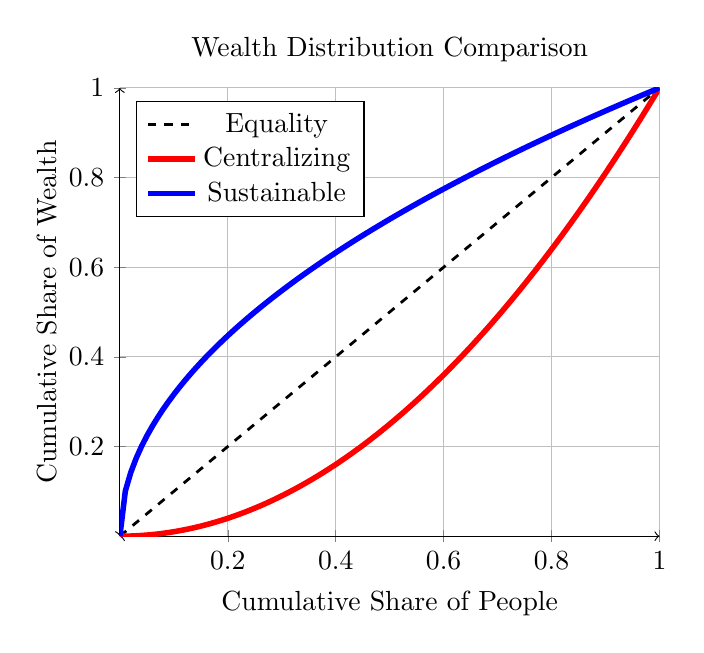
\begin{tikzpicture}
                    \begin{axis}[
                            title={Wealth Distribution Comparison},
                            xlabel={Cumulative Share of People},
                            ylabel={Cumulative Share of Wealth},
                            xmin=0, xmax=1,
                            ymin=0, ymax=1,
                            legend pos=north west,
                            axis lines=middle,
                            axis line style=<->,
                            x label style={at={(axis description cs:0.5,-0.1)},anchor=north},
                            y label style={at={(axis description cs:-0.1,.5)},rotate=90,anchor=south},
                            grid=major,
                        ]
                        % Line of Equality
                        \addplot[
                            color=black,
                            mark=none,
                            dashed,
                            line width=1pt,
                            domain=0:1,
                        ]{x};
                        \addlegendentry{Equality}

                        % Centralizing Incentives Lorenz Curve
                        \addplot[
                            color=red,
                            mark=none,
                            line width=2pt,
                            domain=0:1,
                            samples=100,
                        ]{x^2};
                        \addlegendentry{Centralizing}

                        % Sustainable Incentives Lorenz Curve
                        \addplot[
                            color=blue,
                            mark=none,
                            line width=2pt,
                            domain=0:1,
                            samples=100,
                        ]{sqrt(x)};
                        \addlegendentry{Sustainable}

                    \end{axis}
                    % Your first plot code here
                \end{tikzpicture}
                \caption{First Plot}
                \label{fig:growth-influence}
            \end{minipage}\hfill
            \begin{minipage}{0.45\textwidth}
                \centering
                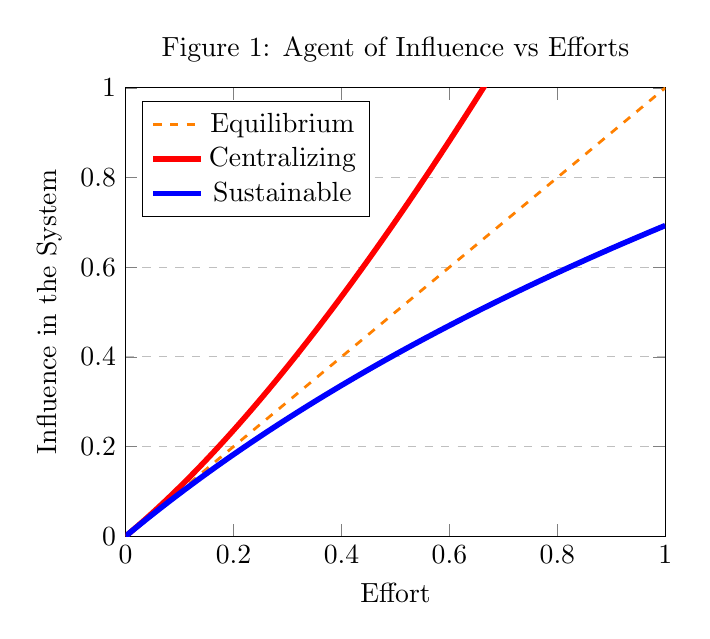
\begin{tikzpicture}
                    \begin{axis}[
                            title={Figure 1: Agent of Influence vs Efforts},
                            xlabel={Effort},
                            ylabel={Influence in the System},
                            xmin=0, xmax=1,
                            ymin=0, ymax=1,
                            legend pos=north west,
                            ymajorgrids=true,
                            grid style=dashed,
                        ]
                        % Linear growth
                        \addplot[
                            color=orange,
                            mark=none,
                            dashed,
                            line width=1pt,
                            domain=0:1,
                        ]{x};
                        \addlegendentry{Equilibrium}
                        % Sub-linear growth (example: square root)
                        \addplot[
                            color=red,
                            mark=none,
                            line width=2pt,
                            domain=0:1,
                            samples=100,
                        ]{x+x*(ln(x+1))};
                        \addlegendentry{Centralizing}
                        \addplot[
                            color=blue,
                            mark=none,
                            line width=2pt,
                            domain=0:1,
                            samples=100,
                        ]{{ln(x+1)}};
                        \addlegendentry{Sustainable}
                    \end{axis}
                    % Your second plot code here
                \end{tikzpicture}
                \caption{Second Plot}
            \end{minipage}
        \end{figure}
        % \begin{multicols}{2}

        \subsection{Recent cryptographic advancements}
        Recent cryptographic advancements have enabled the development of new governance and consensus mechanisms that may be used to address the challenges faced by DAOs. For example, the use of zk-SNARKs (Zero-Knowledge Succinct Non-Interactive Argument of Knowledge) allows for the creation of verifiable and private voting systems that can be used to ensure the integrity of voting processes within DAOs \cite{Ben-Sasson2014}, while MPC threshold-signature protocols can be used to create secure multi-party data signing process \cite{Doerner2023} and fully homomorphic encryption promises us soon ability to run fully private calculation directly on-chain \cite{Fhenix}.\\
        Summing this section up, we can say that whatever new protocol is designed for governance, it is realistic to set requirements of privacy in voting and proposing process.

        \subsection{Proposed Protocol origins}\label{sec:protocol_origins}
        The foundation of this research stems from a game played by a small group of Lithuanian friends in a chat messenger since 2017. Initially designed for leisure and sharing music, this game has unexpectedly exhibited properties desirable in governance protocols.\\
        The game, played by 5 to 10 participants, involves a rotating "game master" role. Each round, participants submit music they enjoy to the game master, who compiles them into a playlist. Participants then vote on their favorite composition, and the game master reveals the results, including proposer identities and scores. The game continues until 100 compositions are added to the playlist, with the final ranking based on accumulated scores\cite{DariusYoutube}.\\
        This game's design inherently resists agenda manipulation due to its mandatory proposal-submission prerequisite for voting, a stark contrast to traditional voting systems vulnerable to small-group dominance\cite{McKelvey1976}. Furthermore, it effectively mitigates negative proposal effects like the Halo effect \cite{Verhulst2010}. \\
        Interestingly, the game demonstrates high participation and retention rates, suggesting potential for adaptation as a governance protocol (elaborated in case study section). The primary limitation lies in participants' inclination towards specific interests (music in this case) or groups of people.

        The game's communication complexity appears to be $O(3n)$ per round, as participants submit a proposal, receive a batch of proposals, and then submit a vote.

        This research aims to build upon this foundation, exploring the game's potential as a scalable, decentralized governance protocol with built-in resistance to manipulation and high participant engagement.


        \subsection{Summing up the context}
        From the issues identified in the background sections we can sum up that there are multiple problems that are faced both on network protocol level governance as well as on application layer built DAOs: Low participation rates, low Nakamoto coefficients (high centralization), lack of application layer commitments, inability to perform time-critical actions autonomously and in decentralized fashion, lack of multidimensional indices needed for knowledge work assesement.\\
        We can also see that incentive based protocols cause centralization when using own governance power equivalent as reward for protocol participation, yet decentralized organizations are not able to provide a commitment mechanism for participants, nor do they have truly autonomous way to appoint stakeholders purely from the mission it has, nor identify competent actors in the system to take prompt, time-critical actions.\\
        Both on consensus layer based on continuous proving and application layer with share-holder voting we identified different problems. To some extend these problems are generic, and explained by lack of ability to autonomously distribute governance power, the recent studies have shown that Initial Coin Offerings (ICOs) are very suspectable to speculations and might be seen as root cause centralization \cite{Johannes24}. This leads to situation where reputable security and venture capital funds suggest new players a "progressive decentralization" approach to coupe with the threats\cite{a16z20}\cite{Webber23}, yet these articles do not offer a sustainable and scalable mechanism for decentralizing and staying efficient.
        We also outlined that already existing DAO precedent can show positive dynamics in Nakamoto coefficient when influence is sub-linear to efforts (or completely absent), compared to Consensus Layer systems that incentivize participants. We also outlined precedent of a game that has high participation rates and user retention (further elaborated in case study section).\\

        \section{Protocol Description}

        In order to enable deductive reasoning, we can outline specifications that a generic abstract organization must fulfill. Besides these, we preferably want to system to be compatible with existing solutions and technologies that allow data integrity, privacy and security, assuming that distributed ledger and multiparty computation signing may be combined to cover these problems. \\
        We are seeking for protocol that is:\\
        \textbf{Mission aligned}: Organization members should actively participate in the decision-making process by the design of the protocol, their activity shall be directly impacting the organization goals and mission.\\
        \textbf{Highly performant}: Ideally, every organization design shall automatically align participants in collaborative model, enabling everyone to do their best contribution towards shared direction, with utilizing full potential of competitive performance provided by decentralized autonomous methodology.\\
        \textbf{Centralization resilient}: Protocol should be designed in a way that over time dependency on single actors shall be reduced, Nakamoto coefficient shall increase, promoting collaboration over competition for those aligned in automatic manner. \\
        \textbf{Multidimensionality}: Protocol should enable multidimensional indexes and foundational models to be built on top of it, as well as promote working groups that can be more operative than a main governing body. At the global scale this should support automatically combining multiple DAOs in superset and enable establishing data, asset and control specific flows-controls.\\
        \textbf{Rational}: Protocol should be designed in a way that any network node must be seen as rational-agent which may diverge from collective interest or collude with others and still not able to reach  influence over the system beyond what protocol accounts for.
        \\

        \paragraph*{}
        In order to define quantitative metrics over these declared values in a most generic way, we will use vector space modelling. Such social embedding is used to refer to the representation of individuals or groups as vectors within a social network. Let's introduce the concept of a agent alignment vector, denoted as  $\vec{A}$. This vector captures the collective preference of the group that can be seen as united entity within a given context, such as publicly announced topic, or any other group member specific property. We can denote such context as global alignment vector as:
        \begin{equation}
            \label{eq:glob-align}
            \vec{G} = \sum_{i=0}^{N_{i}} \vec{A_i} + \vec{C}
        \end{equation} Where $N_i$ denotes total number of such groups at given time and $\vec{C}$ is some predefined context constant value.
        If we assume numerous such possible contexts denoted ${N_j}$, then we also can denote an universal alignment vector describing every possible context $j$ as:
        \begin{equation}
            \vec{U} = \sum_{j=0}^{N_{j}} \vec{G_j}
        \end{equation}

        To define a performance criteria, we can denote time dependency for these vectors, to underscore their ever changing nature of decision making:
        \begin{equation}
            \vec{U(t)} = \sum_{j=0}^{N_{j}} \vec{G_j(t)} = \sum_{j=0}^{N_{j}}(\sum_{i=0}^{N_{i}} \vec{A_{ij}(t)} + \vec{C_j})
        \end{equation}
        In such case, a prompt decision making process,  describing ability for high performance can be seen as derivate function of time:
        \begin{equation}
            \label{eq:speed-of-changes}
            \frac{d\vec{U}}{dt} = \sum_{j=0}^{N_{j}} \frac{d\vec{G_j}}{dt} = \sum_{j=0}^{N_{j}} (\sum_{i=0}^{N_{i}} \frac{d\vec{A_{ij}}}{dt} + \vec{C_j})
        \end{equation}

        Deducting of our requirements, the mission alignment is can be seen as stability of $\vec{U}(t)$ and $\vec{G_j}(t)$ over time, multidimensionality is quantified by ${N_j}$,  participation rates by $N_i$ while centralization by standard deviation of the magnitudes of a set of vectors $\vec{A_{ij}}(t)$ and can be denoted as follows:

        \begin{equation}
            \sigma_{\|\vec{A_{ij}}(t)\|} = \sqrt{\frac{1}{N_{i}N_{j}} \sum_{j=0}^{N_{j}} \sum_{i=0}^{N_{i}} \left( \|\vec{A_{ij}}(t)\| - \mu \right)^2}
        \end{equation}

        where $\|\vec{A_{ij}}(t)\|$ represents the magnitude of the vector $\vec{A_{ij}}(t)$, and $\mu$ is the mean magnitude of the vectors, given by:

        \begin{equation}
            \mu = \frac{1}{N_{i}N_{j}} \sum_{j=0}^{N_{j}} \sum_{i=0}^{N_{i}} \|\vec{A_{ij}}(t)\|
        \end{equation}

        Assuming that $\vec{A}$ represents groups interest, it can be further broken down as the aggregate of individual preference vectors $\mathbf{P_i}$. In such, a group ideal delegate can be defined as a participant whose $\mathbf{P_i}$ aligns most closely with $\vec{A}$.
        This alignment maximizes their positive contribution to the overall group preference and can be quantified using measures like cosine similarity or Euclidean distance between the participant's and the group's vectors.

        The protocol's inclusive and autonomous requirement nature allows to envision that even a fully stochastic process, where participants could be assumed to make random decisions regarding tournament participation, proposals, and voting, an $\vec{A}$ could be defined.
        However, we postulate the existence of an underlying, unknown global alignment vector $\mathbf{G(t)}$, that reflects the overall preferences of all protocol participants across time. \\
        This concept accommodates the diverse preferences of all participants, even in the boundary case of entirely random decisions.
        In this fully stochastic scenario, the group's alignment is characterized by entropy, a measure of randomness. The Euclidean distance of each member's rank from the most probable rank for a random participant can serve as a measure of their capacity for random decision-making. \\
        Conversely, in non-stochastic processes, participants exhibit alignment towards an arbitrary direction, shaped by their free-will choices to join specific groups and context. The protocol goals hence can be seen as to quantify these vectors and ensure their desired properties.


        \subsection{Transferability}
        \label{sec:transferability}
        In order to support solving all of the objectives, we propose to specify, that outcome of protocol is a transferrable asset, that can effectively tokenize the competence rating of bearer.
        Transferability is an important aspect as this allows free market rules to establish and accomplish multiple goals, starting with agent rational actions: even concepts of corruption and collusion can be seen as game-theoretic \cite{Macrae1982}, are not necessarily bad \cite{Leff1964}, and can be seen trough definition of an intrinsic value of any transferable asset. Other words saying, we see personal competences in CPSS frameworks useful as a market value, that may be useful to trade. \\While this can be argued as a controversial statement, we can discuss that in the real world competence indeed is often traded in form of a investing time and money in education, relationships, that eventually form a social ranking. Since we declare as a requirement to have a compounding resistance, it forms a solid basis for building economic models that penalize competence-market participants heavy enough,  so that competence is not traded in a way that it can be easily bought by a single entity.
        Transferability of value opens vast application opportunities, as other protocols are free to define staking commitments with specific slashing rules, similarly as PoS consensus mechanisms do, therefore bringing one of the lacking consensus layer features on-to on-chain governance. Eventually, this helps forming a rational economic model that would incentivize any participant to treat his rating in a similar careful and responsible manner, as one does with his assets.\\
        With such, we envision that both ${\vec{A}}$ and ${\vec{G}}$ may be tokenized separately, whilst there is connection between these, reciprocity is not a strict requirement, meaning that while conversion of ${\vec{A}}$ into ${\vec{G}}$ must be supported by protocol as per Eq. \ref{eq:glob-align}, the reverse exchange can be left for a free market to decide upon, leaving some extra space for protocol incentives design which we will use in following sections to create additional useful properties for the protocol.
        Nevertheless, transferability does not exclude any applications where such rating asset must be locked. Use cases of ownership within Account Abstraction\cite{Qin2023} model could be designed to ensure asset is non-transferable and acts as account-bond proof of competence if such an use case would be desired.\\
        Token economics,and their application in governance systems are widely used today, however mechanisms such as Initial Coin Offerings (ICOs) have shown to be a weak spot as this opens doors for bad entrepreneurs \cite{Johannes24}, and as already discussed in background section, ultimate outcome of such allocation is extremely centralized, and suspect of issues such as centralization and inability to perform well.

        \subsection{Ranking ladder}

        Providing a resistance to influence compounding becomes a critical aspect part for such protocol, since we are relying to a free-market values and principally do not require any specific identity solution as a dependency to this protocol.
        Our foundational model for this resistance lies in extending  ~\ref{sec:protocol_origins} idea, to introduce \textit{ranking ladder} (Fig. \ref*{fig:game-connection}) that lets game winner to participate in next game with higher level of rewards only if it holds an asset of rank below.Such architecture allows to design initially low ability to influence ${\vec{G}}$ and exponentially increase as participant succeeds climbing up ladder. As participants gain higher ability to influence global alignment value, quantitative measure of that is their individual preference vector magnitude $|P|$, which protocol will account for increasing only as they prove to be the most impactful part of their group $|A_i|$.
        \documentclass{article} % Use an appropriate document class for your main document
\usepackage{tikz}
\usetikzlibrary{positioning, shapes.geometric}

\begin{document}

\begin{figure}[ht]
    \centering
    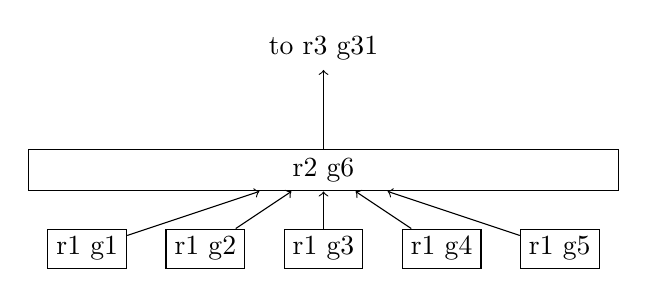
\begin{tikzpicture}[node distance=1cm and 1cm]
        % Bottom level blocks (5 participants)
        \foreach \x in {1,...,5} {
            \node[draw, rectangle, minimum width=1cm, minimum height=0.5cm] (P-\x) at (\x*1.5, 0) {};
            % Add "Rank X" text inside each block
            \node at (\x*1.5, 0) {r1 g\x};
        }

        % Single block for the game
        \node[draw, rectangle, minimum width=7.5cm, minimum height=0.5cm] (Game) at (4.5, 1) {r2 g6};

        % Connect participants to the game
        \foreach \x in {1,...,5}
            \draw[->] (P-\x) -- (Game);

        % Arrow pointing upwards from the top block with text "to r3"
        \draw[->] (Game.north) -- ++(0,1) node[above] {to r3 g31};
    \end{tikzpicture}
    \caption{Diagram illustrating the rank ladder. With minimum participant requirements of 5, 30 games are required to create a rank 3 game. Strong candidate would need only 2 wins to reach it.}
    \label{fig:game-connection}
\end{figure}


\end{document}
        Participant rank $R$ hence represents such quantization of $|A_i|$:

        \begin{equation}
            \label{eq:comp-quant}
            R = Q(|A_i|)
        \end{equation}
        To further introduce compounding resistance, we define protocol ladder climb event requirement: previous ladder step tokenized element must be removed (exchanged) in order to obtain higher ladder rank.


        In order to see how this affects protocol parameters on practice, we can analyze a sybil attack scenario, which is one of most prominent threads for any permissions less protocol that produces intrinsic value.


        If each game requires a commitment, such as a participation fee, we can demonstrate that the proposed ranking ladder introduces a desired non-linear compounding friction for potential malicious actors attempting to manipulate the system.

        To illustrate this, let's use the concept of a agent alignment vector introduced in Eq.(\ref*{eq:glob-align}). In the absence of collusion or manipulation, a blind proposing-voting process is inherently probabilistic, where the inverse of groups  magnitude $|\vec{A}|$ quantifies the resistance to entropy inherent in participants' choices.


        Any colluding actors attempting a Sybil attack are effectively trying to manipulate this global alignment vector $\mathbf{G(t)}$. Given our earlier requirements for an ideal protocol, it should encourage the formation of small groups while maintaining a large overall active participant count. This breakdown into smaller groups serves as a pre-alignment mechanism, as participants willingly choose to collaborate. In this context, any group can be seen as colluding, with Sybil attacks representing an extreme case of such alignment.

        Therefore, from the outset, each group is inherently aligned towards a specific direction, determined by the free will of its members to participate in a particular tournament. This pre-alignment introduces a degree of predictability, quantified by $|\vec{A}|$, into an otherwise stochastic process.


        If there is a game fee, that creates participation resistance, we can say that achieving a specific level of competence cost is $\$R$ and can be expressed as a function of level of competence $i$ and game fee $X_g$ and mathematical expectation for costs achieving specific rank via sybil attack described as
            \begin{equation}
                \mathbb{E}[\$R] = X_g \cdot \mathbb{E}[N_{\text{sybils}}(R)]
            \end{equation}

            % $$\mathbb{E}[\$C(i)] = X_g*\mathbb{E}[{N_{sybils}(i)}]$$

            Where $N_{sybils}(R)$ is a number of sybil accounts required to win a game, and hence obtain rank $R$. Due to tournament fragmentation, an attacker mixing Sybil accounts with fair players must strategically allocate Sybils across games for cost efficiency. However, this is challenging due to each group's unique $\vec{A}$, finding suitable games for manipulation is difficult.  Meanwhile, from a deductive reasoning, the distance between fair actors' preferences $P_i$ and $\mathbf{G(t)}$ should diminish as their rank increases, reflecting the protocol's design of identifying participants alignment.


            This means that for any protocol participant, confidence over group conducting a sybil attack will increase as level of games increase, hence they will be more likely to refuse joining games with such, resulting
            \begin{equation}
                \lim_{R \to \infty} \frac{\mathbb{E}[N_{\text{sybils}}(R)]}{R} = N_{\text{min}}
                \label{eq:limit-nmin}
            \end{equation} Where $N_{min}$ is amount of peers required to join the game. Hence, a straightforward Sybil attack scenario where the attacker attempts to manipulate the protocol by flooding games with multiple Sybil accounts may be analyzed.
            Then for an attacker who tries to conduct a sybil attack it would cost
            \begin{equation}
                \$R = X_g*N_{min}^R
            \end{equation}
            to get rank of level $i$. At the same time, for the agent who is relying on his pure competence and wins each game, same cost would be only \begin{equation}
                \$R = X_g*R
            \end{equation}
            In the context of governance power, this allows to draw price relationship between governing competence power that may be put at stake, and total value loked (TVL) at stake:
            \begin{equation}
                TVL << \$R
            \end{equation}

            Total value locked must be substantially lower then a cost for obtaining rank due to reason that empirical studies are needed to see how fast will required sybil count converge (Eq. \ref{eq:limit-nmin}) in practice. which strongly depends on how much stochastic process is inherit in such voting system. Additionally sybil resistance will benefit greatly from use of quadratic voting systems which already shown to be helpful in blockchain governance field \cite{Buterin20}\cite{Benhaim2024}.


            \subsection{Time constraint}
            \label{sec:time-constraint}

            As discussed in the previous section, any overt Sybil attack requires multiple game rounds to establish a sufficient ranking within the system. In the original protocol, participants engage in several voting and proposing rounds to determine a winner.

            We preserve this multi-round requirement to enhance protocol security, ensuring resistance to centralization and maintaining mission alignment. We introduce a time constraint,  $t_c$ which represents the minimum time needed to mint a single competence asset of any rank.
            Therefore, the intrinsic value of a tokenized competence rating is determined not only by financial effort and success among peers but also by the time invested in continuously improving one's position within the system. Even with parallel attack instances, an attacker would still require $t_{attack}(R) = t_c \cdot R$ time to reach rank $R$. This extended duration allows protocol members ample opportunity to detect and respond to the attack. Similarly, the $t_c$ may be broken down to smaller components, giving participants ability to leave or cancel a game, specify round times etc.


            \subsection{Composable architecture}
            The DAO hack\cite{Liu2021} a single entity governing on-chain operations creates a central point of failure. Even with a theoretically perfect design, a single governing body struggles to match the versatility, adaptability of smaller groups is desired \cite{Buterin22}.  This highlights the necessity of multidimensionality to achieve a robust, global DAO concept while maintaining high performance.
            Furthermore, the time constraints discussed in Section \ref{sec:time-constraint} imply that changes in ${\vec{G_j}}$ (Eq.\ref{eq:speed-of-changes}) should be gradual, even under ideal conditions.
            To address these challenges, we propose a composable architecture where each potential ${\vec{G_j}}$ operates as an independent DAO. This eliminates single points of failure and enables the parallel emergence of successful solutions.

            A non-permissive rating system, tokenized via rating representation $R$, empowers competent participants by amplifying voting power or granting specific permissions within an organization or contract. The global, distributed DAO $\vec{U}$, emerges as the aggregate of all $G$, representing a theoretical value not elaborated upon in this work. \\
            Participants gain subject-specific competence $R_{j}$, which determines governance weights ($W_j$) within the corresponding DAO: $W_j = f(R_{j})$. As $R_j=f(t_c)$ (time-dependent), resulting weights are also time-dependent: $W_j=f(t_c)$. The protocol facilitates the transformation of $R_j$ into $W_j$.
            \\From Eq. \ref{eq:glob-align} and Eq. \ref{eq:comp-quant} it is possible to infer that protocol must provide means of transforming  to such DAO governance weights $W_j$.  This been already discussed in Sec. \ref{sec:transferability} that such conversion does not require to be reciprocal, meaning that reverse conversion may be market defined. This is a useful property as multiple financial and market instruments may be designed to ensure stimulus for participants to pursue their success strategy within the protocol.  \\ 
\usetikzlibrary{arrows.meta, positioning}

\begin{figure*}

\begin{tikzpicture}[
    node distance=2cm,
    every node/.style={draw, align=center},
    arrow/.style={-{Latex[length=3mm, width=2mm]}, thick}
]


% Single block for the game

% Nodes
\node (competence) {Competence \\ $C_{j}$};
% \node[draw, rectangle, minimum width=7.5cm, minimum height=0.5cm, below=of competence] (Game) {r2 g6};
% Bottom level blocks (5 participants)
\foreach \x in {1,...,5} {
    \node[draw, rectangle, minimum width=1cm, minimum height=0.5cm, below=of Game, xshift=(\x-5)*1.2cm] (P-\x) {};
    % Add "Rank X" text inside each block
    \node [below=of Game, xshift=(\x-5)*1.2cm] {r1 g\x};
}
\node (exchange) [right=of competence] {Unidirectional \\ Asset Exchange \\ $P_g = f(C_{j})$  };

\node (DAO) [right=of exchange] {DAO \\ ${G_j(t)} = \sum_{i=0}^{i_{\text{max}}} P_g$ };
\node (quorum) [below=of DAO] {Quorum Group \\ $V_{aj}$};
\node (dao) [below=of quorum] {DAO \\ $G_j(t)$};
\node (market) [below=of dao] {Market Value \\ Increase};

% Connect participants to the game
\foreach \x in {1,...,5}
    \draw[->] (P-\x) -- (competence);

% Arrow pointing upwards from the top block with text "to r3"
% \draw[->] (Game.north) -- ++(0,1) node[above] {to r3 g31};

% Arrows
% \draw [arrow] ()
\draw [arrow] (competence) -- (exchange);
\draw [arrow] (exchange) -- (DAO);
\draw [arrow] (DAO) -- (quorum);
\draw [arrow] (quorum) -- (dao);
\draw [arrow] (dao) -- (market);



% Labels
\node [above=0.5cm of competence] {Competence Minting};
\node [above=0.5cm of DAO] {Governance Power Function};
\node [above=0.5cm of quorum] {Quorum Group Formation};
\node [above=0.5cm of dao] {DAO Representation};

\end{tikzpicture}

\end{figure*}
            \paragraph{Exit Strategies and Governance Transitions.}
            Existing DAO frameworks can leverage fungible tokens derived from $R_{j}$ through a unidirectional asset exchange. This enables high-scoring participants to "exit" and convert their competence into governance power within the underlying DAO, essentially forming a specialized "guild" (Fig. \ref{fig:competence-transfer}).
            While the rating asset $R$ holds intrinsic value, high-scoring participants may stagnate at the top due to a lack of competition. Additionally, tokenized ratings are better suited for reputation representation than direct governance, as they are vulnerable to unforeseen losses during possible third party staking. The exchange into governance weight $W_j$ symbolizes a transition from service provision (risking reputation) to a managerial role, where participants focus on generating intrinsic value for the DAO.
            \paragraph{Exponential Rewards and Sybil Attack Mitigation.}
            To incentivize participation and prevent stagnation, exponential rewards are necessary, especially for higher ranks with fewer participants. Governance power must also account for potential sybil attacks:
            \begin{equation}
                W_{gj}(R) \propto  X_{g_j}*\mathbb{E}[N_{sybils_j}]^{R_j}
            \end{equation}
            Where $\mathbb{E}[N_{sybils_j}]$ is expectation of required $N_{sybils}$. If a group of high-scoring participants exits, they're likely to gain substantial power in the underlying DAO, whose reputation is established from past rounds. This aligned group effectively represents $G_j(t)$  at a specific time when they achieve quorum.

            \paragraph{DAO Dynamics and Evolution.} The original protocol competence generation algorithm stay unaffected and already established uses for competence rating system with asset of $R$ are unaffected by the new governance power distribution of $W_j$. However, the new DAO quorum can define $G_j(t)$ for their specific subset and control the organization's public descriptions and URIs. This incentivizes the new DAO to increase its market value, justifying the exit strategy and driving demand for the $X_g$ asset needed for $W_j$.\\
            The Nakamoto coefficient increases over time as new participants enter and gain power. Early adopters can maintain control by strategically acquiring lower-ranking members' $R_{j}$, creating a reverse market that balances $R$ to $W_j$. Active participation is crucial for maintaining power in the face of inflation and new entrants.
            \paragraph{Composable DAO Framework and Network Effects.}
            A composable DAO framework emerges when a high-scoring group deploys another autonomous competence protocol with a subsidiary DAO, linking both to a shared asset holding contract such as new multisignature wallet. TThis effectively splits the organization, with asset ownership tied to the original but governance shared between the two bodies. The derived protocol cost can be linked to the parent DAO ($ \grave{X}_{gj}$ to $G_j$), , forming a network of interconnected DAOs (Fig. \ref{fig:dao-composition}).



            This architecture offers a decentralized, scalable, and adaptable governance model, incentivizing participation and excellence while mitigating centralized control and stagnation risks.


            \subsection{Privacy constraints}

            This paper addresses privacy requirements in a proposal evaluation protocol. The protocol aims to balance transparency and anonymity by:
            \begin{itemize}[nosep]
                \item Linking Proposals to Proposers: Enabling the association of proposal submissions events with specific proposers, without revealing the proposal content initially.
                \item Verifying Proposal Uniqueness: Ensuring the submitted proposal was uniquely known to the proposer at the time of announcement, while preserving proposer anonymity.
                \item Protecting Preference Selection: Safeguarding the privacy of participant preferences during proposal selection.

            \end{itemize}
            \paragraph{}

            These measures aim to mitigate the Halo effect \cite{Verhulst2010}, where judgments are influenced by personalities rather than ideas, and deter strategic voting by increasing the complexity of coordinated attacks against competent proposals. The de-personalized voting process aims to foster a fairer evaluation environment by focusing on the merit of the proposals themselves.
            % \end{multicols}

            % \paragraph{}
            % \begin{multicols}{2}

            % Concluding this section, we advocate that multidimensionality and free-market values will provide a way to ensure high participation rates, as participants will be able to participate in the decision-making process in a category that they are interested in, grouping with like-minded people in the fields they are competent in, and lastly - are rewarded for being in.
            % With a ranking ladder, and a multidimensional representation, this can be seen as a global framework for building education and helping young talents to discover their path by observing very well quantized data on their progress. \\ We may also suggest that this protocol functionally may be presented as simply a new way of talking, where each input - seen as valuable idea, and each vote - seen as a valuable feedback, and each game final, as actionable result.\\
            % In order to support such high participation rates, the user experience must be ensured as simple as possible, and the application must be designed in a way that it is easy to use and understand. In order for that, we require to have extensive metadata available for user experience purpose by the protocol as key requirement. For example, when participant sends in encrypted vote, or proposal - protocol shall be able to publicly announce that particular participant has submitted a vote, while not revealing the content of the vote nor the linkage to it after content is revealed for voting.\\
            
\usetikzlibrary{arrows.meta, positioning}

\begin{figure*}

    \begin{tikzpicture}[
        node distance=2cm,
        every node/.style={draw, align=center},
        arrow/.style={-{Latex[length=3mm, width=2mm]}, thick}
        ]


        % Single block for the game

        % Nodes
        \node (Competence_A) {Ranking System A};
        \node[right of=Competence_A, , xshift=2cm]  (A_token) {Gov. Token "A" \\ $Wj(t)$};
        \node[above of=A_token]  (DAO_origin) { DAO "A"};
        \node[above of=DAO_origin] (Multisig) {Multisig M of N};
        \node[right of=A_token, xshift=2cm] (exchanger) {$X_{gb} = f(W_j(t))$};
        \node[right of=exchanger, xshift=2cm] (Competence_B) {Ranking System B};
        \node[above of=Competence_B]  (B_token) {Gov. Token "B"};
        \node[above of=B_token]  (DAO_B) { DAO "B" };

        \draw [arrow] (Competence_A) -- (A_token);
        \draw [arrow] (A_token) -- (DAO_origin);
        \draw [arrow] (DAO_origin) -- (Multisig);
        \draw [arrow] (A_token) -- (exchanger);
        \draw [arrow] (A_token) -- (exchanger);
        \draw [arrow] (exchanger) -- (Competence_B);
        \draw [arrow] (Competence_B) -- (B_token);
        \draw [arrow] (B_token) -- (DAO_B);
        \draw [arrow] (DAO_B) -- (Multisig);






    \end{tikzpicture}
    \caption{Diagram describing progressive decentralization via DAO composition. As initial group governing DAO "A" experiences inflation it may provision next organization "B" to focus on specific aspects of arbitrary protocol, and maintain any asset security by moving them further on to the governance  chain. If such assets are assigned to multisig, original DAO value is preserved, therefore allowing organization to grow both horizontally and vertically.  }
    \label{fig:dao-composition}
\end{figure*}
            % Write your conclusion here
            \section{Implementation}
            Protocol particular implementation may vary depending on environment and requirements, however we can outline a generic implementation that can be used as a reference for further development. Following reference describes implementation as a smart contract on Ethereum Virtual Machine compatible network.
            \paragraph{Rating asset}
            is semi-fungible tokenized asset contract, such as defined by ERC1155\cite{EIP1155} interface standard and with emission permit granted only to contract(or contracts), that implements autonomous rating identification. Participation fee $X_g$ is expressed as ERC20\cite{EIP20} token interface which may represent a overseeing organization governance power.
            Privileged methods available to rating identification contracts: minting new token, burning existing token from owners balance.

            \paragraph{Competence identifaciton contract}
            operates by logic that is given in (Algorithm \ref{algo:basic-acid}). The specific rules of produced by autonomous decision making based on competence identification goals, may be specific for goals. For example, if goal is to formulate one, finalized proposal over multiple round, a later rounds based proposals could be seen as more refined and hence applied higher weights.
            % \end{multicols}

            % \begin{multicols}{2}

            \paragraph{DAO, Governance Token \& Multisig}
            can be used from already established frameworks for token based voting may be used. Various frameworks for DAOs are available\cite{AragonOSx}\cite{OpenZeppelinGovernor}, as well as industry standard multisignature wallet\cite{GnosisSafeMultisig}. In standard implementation we suggest requiring $2/3$ quorum threshold on the multisignature wallet.

        \paragraph{Game Master concept} is needed to provide privacy. The game master is responsible for collecting proposals and announcing fact of activity without disclosing the actor, then posting them as batch to a competence identification contract, collecting votes in a similar manner, without tell nor who, nor for whom votes, and finally revealing the results.\\ This is potential failure point as such agent may disclose or even attempt to corrupt data. Whilst in our simple implementation a trusted backend server is used, an ideal solution can be achieved by multiparty computation, where every participant seen as network participant that can sign transactions with encrypted data, and decrypt it according to the protocol requirements. Fully on-chain fully-homomorphic encryption promised by emerging blockchains poses interest\cite{Fhenix}.


        % Write your results here
        \section{Case Study}
        \subsection{Original Concept: A Music-Sharing Game}
        To gather empirical data, we analyzed a group's activity and historical records in a music-sharing game \cite{DariusYoutube}. Participants share YouTube music clips, forming playlists. From 2017 to 2023, 17 games were played, each averaging 13 turns, 8 participants, and 3 months duration. Roughly 1700 proposals and votes were recorded, with a 100-song playlist limit per game.\\
        Over the years, 34 participants joined, 22 completing at least one tournament and 15 completing at least two. Of the original 6 players, 3 remain active, with 8 active users in the latest game. Non-voting instances were negligible, below 5\% of all votes. \\
        Despite lacking explicit incentives and requiring effort as occasional game masters, participation rates were remarkably high:
        \begin{itemize}[nosep]
            \item \textbf{Participation rate} of 95\% for active users
            \item \textbf{User retention} for three month period of 65\%
            \item \textbf{User retention} for two tournaments and roughly six month of 44\%
            \item \textbf{User retention} after 72 month of 9\%
            \item Average of \textbf{8 proposals and votes per user} per annum
        \end{itemize}

        The low absolute numbers however are explainable by user complex manual score calculation process and closed community by itself which never oriented itself towards big growth and hence let to do assertion that could be even higher on a well designed automated protocol.

        We also observed that collected playlists, ordered by high-score compositions, are of high quality and form a good representation of participants' preferences, while the winner of the tournament is often a participant that is able not simply propose a popular song, but to propose a song that is liked by many participants, including such aspects that participants will likely vote songs they hear for the first time (original ideas).

        \subsection{Prototype study}
        We wrote a simple implementation of such game that allows ease game process with game automation. Two games games were conducted each game consisted of 9 participants. Participants included original concept participants and random people who did not know each other of different age groups. Game rules and requirements were set close to original: participants were required to send URLs for music on youtube with composition length of no more than 10 minutes and had to listen for all of them in order to make a vote. Privacy constraints were ensured by a backend server. Quadratic voting system was used, allowing users to spend 14 vote credits in integer form. Only notable difference  was that for sake of design simplification, the total playlist length was replaced with fixed round count.\\
        Participants were given no incentives, and most of the group had no prior blockchain experience nor significant interest in it.\\
        Some participation rate metrics were recorded during these two games:
        \begin{itemize}[nosep]
            \item \textbf{Participation rate} of 84\% for active users
            \item \textbf{User retention} of 66.7\% after first game
            \item Average of \textbf{3.23 proposals and 3.09 votes per user} per month
        \end{itemize}

        Based on conducted experience, participants were asked to fill feedback form, questions asked was possible to rate from 0 to 5.
        \begin{itemize}
            \setlength\itemsep{2px}
            \item \textbf{Overall experience rating:} 88\%.
            \item \textbf{Resulting playlists rating:} 92\%.
            \item \textbf{\textit{"Did playing this game give you new insights into the personalities or perspectives of other players?"}}: was rated at 80\%.
            \item \textbf{\textit{"Would you be willing to play such game with your friends or family?"}}: was rated at 84\%.
        \end{itemize}
        Out from participants that left game could be noted significant age, and preference difference
        Participants also proposed various different game topics and generally expressed interest. \\When asked \textit{"If you missed any turn to vote or propose, what were main causes"}, all respondents answered that they enjoyed the process however lacked time to listen all of the compositions.



        \section{Potential Applications}
        \paragraph*{Better ICOs:} By releasing an ERC20 token as payment for competence games, projects can create a more meritocratic system where participants earn governance tokens based on their demonstrated skills and contributions. This approach aligns incentives, rewards active engagement, and fosters a community of competent stakeholders who are genuinely invested in the project's success.

        \paragraph*{Autonomous Code-Writing:} In software development, the autonomous competence identification protocol can revolutionize the code-writing process. By treating each round as a programming cycle, developers can submit pull requests, vote on the best solutions, and iteratively refine the codebase. The fixed cycle length ensures a strict deadline, promoting efficiency and focus. The protocol's ability to weight later rounds more heavily acknowledges the cumulative improvement of code over time, incentivizing continuous participation and innovation. Participants are encouraged to actively contribute new code and solutions rather than just reviewing and commenting, fostering a proactive and collaborative development environment.

        \paragraph*{Cross-Stream Collaborative Integrations:} Continuous opinion exchange nature of the protocol can be used to create a seamless platform for cross-stream collaboration and feedback gathering. This reduces the need for time-consuming meetings and calls, enabling teams to collaborate more efficiently and effectively. By fostering a culture of continuous feedback and iterative improvement, the protocol can enhance communication, streamline decision-making, and drive innovation across various streams within an organization.

        \paragraph*{Decentralized Social Networks:} the protocol could assess the quality and relevance of user-generated content, such as posts, comments, and shares. By assigning higher rankings to valuable contributions, the protocol can incentivize users to create meaningful content and discourage spam or low-effort posts. Additionally, it can help identify influential users based on their consistent engagement and the quality of their interactions, fostering a more meritocratic and engaging social media environment

        \paragraph*{Academic Research and Peer Review:} The traditional peer-review process often suffers from biases, delays, and lack of transparency. The autonomous competence identification protocol can address these issues by creating a decentralized peer-review system. Researchers can submit their work, review others' submissions, and receive ratings based on the quality and thoroughness of their reviews. This approach can lead to faster, more objective, and transparent peer review, ultimately improving the quality and credibility of academic research.

        \paragraph*{Online Education and Skill Assessment:} The protocol can be applied to online education platforms to assess and certify learners' skills. By participating in competence games or challenges, learners can demonstrate their knowledge and proficiency in various subjects. The protocol's ranking system can provide a verifiable and transparent way to assess skills, enabling learners to showcase their expertise to potential employers or educational institutions.

        \paragraph*{Prediction Markets:} The autonomous competence identification protocol can enhance these markets by identifying participants with a proven track record of accurate predictions. By assigning higher weights to their forecasts, the protocol can improve the overall accuracy and reliability of the market's predictions. Additionally, it can incentivize participants to continuously improve their forecasting skills to earn higher rewards.

        \paragraph*{Decentralized Autonomous Organizations}: DAOs can utilize the autonomous competence identification protocol beyond governance to enhance various internal processes. For instance, the protocol can be employed to allocate resources efficiently by identifying members with the most relevant expertise and experience for specific tasks or projects. This ensures that resources are directed towards individuals who are most likely to utilize them effectively, maximizing the DAO's overall productivity and impact.

        Furthermore, the protocol can be used to assign tasks within the DAO by matching members' skills and interests with the requirements of different roles or responsibilities. This can lead to a more motivated and engaged workforce, as members are more likely to excel in tasks that align with their strengths and passions.

        Additionally, the protocol can be instrumental in evaluating proposals for new projects or initiatives within the DAO. By assessing the competence and track record of the proposers, as well as the potential impact and feasibility of their ideas, the DAO can make more informed decisions about which projects to pursue, increasing the likelihood of success and minimizing risks.

        \paragraph*{Empathic Agenda and AI Applications:} protocol establishes a framework for rating both participants and ideas, decoupling evaluation from personal biases. Its continuous feedback loop, utilizing previous round results, fosters deeper alignment among participants and cultivates empathy as they iteratively refine their understanding of collective preferences.

        Beyond interpersonal empathy, this property holds significant value for Cyber-Physical-Social Systems (CPSS). By benchmarking AI agents participating in these games, the protocol generates feedback and historical data that can be used to create robust, personalized machine learning frameworks.

        \section{Conclusion}

        This paper has presented a novel protocol for establishing ranking systems in DAOs and consensus-building protocols, aiming to address challenges such as low participation, centralization, and lack of commitment mechanisms. By incorporating a competence-based approach, tokenized ratings, and a composable architecture, the protocol fosters a more engaging, equitable, and secure decision-making process. The real-world case study demonstrates the potential of this approach to drive high participation and retention rates, even without explicit incentives.

        Future research could explore the development of more sophisticated economic models and incentive structures to further enhance participation and mitigate risks. Additionally, the protocol's applicability could be investigated in various domains beyond music sharing, such as decentralized finance, social networks, and scientific collaboration. By bridging the gap between formal consensus mechanisms and subjective human decision-making, this research contributes to the ongoing development of more effective and inclusive governance models for the digital age.



        \clearpage
    \end{multicols}
    % \appendix
    % \section{Appendix A: Listings}
    % 
\begin{algorithm}
\caption{Basic Autonomous competence identification}
\begin{algorithmic}[1] % Enables line numbering
\State \textbf{Prerequisites:} Minimal group size $N_{min}$, Time constant $t_{c}$, Participation cost $X_g$, Competence Asset $C_i$, Protocol Treasury $T$, Minimal turn count ${M, M > 2}$
\State \textbf{Process:}
\Procedure{Preparation}{}
    \State Instance is created at timestamp $t_0=t$, with creators personal join requirements $X_a$
    \State Participants join the group and lock in a commitment: $N_{min} \times (X_g+X_a) \rightarrow T$
    \State Joining period ends at $t_1  \ge t_c + t_0$
\EndProcedure
\Procedure{FirstTurn}{}
    \While{$t_1 + t_c \ge t$}
        \If{new Proposal}
        \State Record ${P_i}$
        \State Record $i$
        \EndIf
    \EndWhile
    \If{Group is full or joining timeout}
        \State Members exchange encrypted proposals (MPC).
    \EndIf
\EndProcedure
\Procedure{DecryptProposals}{}
    \If{Timeout or all proposals received}
        \State Members decrypt proposals using threshold encryption.
    \EndIf
\EndProcedure
\Procedure{RegularTurn}{}
    \State Submit new encrypted proposals.
    \State Submit encrypted votes and zk-proof of valid vote.
\EndProcedure
\Procedure{CalculateRoundScores}{}
    \If{Round ends or all votes \& proposals submitted}
        \State Use TSS cryptography to decrypt everything.
        \State Calculate round scores.
    \EndIf
\EndProcedure
\Procedure{RepeatUntilXProposals}{}
    \State Repeat steps 3-5 until a total of X proposals.
\EndProcedure
\Procedure{FinalizeRankings}{}
    \State Count total votes and sort proposals.
\EndProcedure
\end{algorithmic}
\end{algorithm}


    % \clearpage
    \bibliographystyle{ieeetr}
    \bibliography{whitepaper.bib}

    \clearpage\end{CJK}
\end{document}
